\section{Polynomial Multiplication}
\begin{itemize}
	\item Earlier, we talked about multiplying numbers and also matrices quickly. Today, we'll talk about manipulating polynomials.
	\item Given two polynomials \( p(x) \) and \( q(x) \), what are the fastest algorithms that add and 
		multiply the two polynomials together?
\end{itemize}
\subsection{Representing Polynoimals}
\begin{itemize}
	\item Typically, we'd write a degree \( n-1 \) polynomial as 
		\( p(x) = p_0 + p_1x + p_2x^2 + \cdots + p_{n-1}x^{n-1} \). This is called
		the \textbf{coefficient representation}, represented by an array of numbers \( (p_0, p_1, \cdots, p_{n-1}) \). 
		Note that \( p_i \) 
		 are \textit{real numbers}, not necessarily integers.  
	 \item We will think of \( n \) as being very large, say \( n = 10^{10} \), while thinking that \( p_0, \cdots, p_{n-1} \)
		 to be very small. So we'll imagine that all these arithmetic operations are going to take \( O(1) \) time.  
	 \item Goal: measure runtime as a function of \( n \), not on the coefficients themselves.    
\end{itemize}
\subsection{Adding Polynomials}
\begin{itemize}
	\item Given two polynomials \( p(x) \) and \( q(x) \), we want to output \( r(x) = p(x) + q(x) \), in its coefficient 
		representation. 
	\item How fast can we do this? To find the coefficients of \( r(x) \), we just add \( r_i = p_i + q_i \), and since each 
		takes constant time, there are \( n \) additions, hence \( O(n) \). 
	\item This is like adding integers, but even simpler, since there is no carry over term!
\end{itemize}
\subsection{Evaluating Polynomials}
\begin{itemize}
	\item Given an input \( p(x) = p_0 + p_1x + p_2x^2 + \cdots + p_{n-1}x^{n-1} \), and a real number \( \alpha \in \mathbb R \). 
	\item We want to output \( p(\alpha) = p_0 + p_1\alpha + p_2\alpha^2 + \cdots + p_{n-1}\alpha ^{n-1} \in \mathbb R \). 
	\item How fast can we do this? There are three algorithms that take \( O(n^2) \), \( O(n \log n) \), and \( O(n) \) 
		respectively. We'll first take a look at the \( O(n^2) \) and the \( O(n) \) ones. 
		\begin{itemize}
			\item Algorithm 1: We compute the terms individually and add them together: 
				\begin{align*}
					&\phantom{+a} p_0 & \text{0 multiplications}\\
					&+ p_1 \cdot \alpha & \text{1 multiplication}\\
					&+ p_2 \cdot \alpha \cdot \alpha & \text{2 multiplications}\\
					&+ p_3 \cdot \alpha \cdot \alpha \cdot \alpha & \text{3 multiplications}\\
					&\vdots\\
					&+ p_{n-1} \cdot \alpha \cdot \alpha \cdots \alpha & \text{\( n-1 \) multiplications}\\
					&\rule{4cm}{0.6pt}&\\
					&p(\alpha) & \text{\( O(n^2) \) multiplications}
				\end{align*}
			Notice the repeated computation we have here: when we compute \( \alpha^3 \), we don't actually need to multiply
				\( \alpha \) three times, since we've already computed \( \alpha^2 \) in the previous step. 
			\item Algorithm 2: Initialize an array \( A \), and set \( A[i] = \alpha \cdot A[i-1] \) for each 
				\( i = 1, 2, \dots \). Therefore,  \( A = [1, \alpha, \alpha^2 , \alpha^3, \cdots] \). So every step here 
				takes 1 multiplication, so to compute the whole array \( A \) takes \( O(n) \) steps. Now, if we were to evaluate 
				now:
				\begin{align*}
					&\phantom{+a} p_0 \cdot A[0]& \text{1 multiplication}\\
					&+ p_1 \cdot A[1]& \text{1 multiplication}\\
					&+ p_2 \cdot A[2] & \text{1 multiplication}\\
					&+ p_3 \cdot A[3] & \text{1 multiplication}\\
					&\vdots\\
					&+ p_{n-1} \cdot A[n-1]& \text{1 multiplication}\\
					&\rule{4cm}{0.6pt}&\\
					&p(\alpha) & \text{\( O(n) \) multiplications}
				\end{align*}
				Therefore, this will take \( O(n) \) total steps, hence an \( O(n) \) runtime.  

				\comment{Note here that \( n \) (the problem size) refers to the length of the polynomial, and not the size 
					of the coefficients \( p_i \). We assume these to be small for our analysis, but this is not true in practice, 
				and these computations will add up.}
		\end{itemize}
\end{itemize}
\subsection{Multiplying Polynomials}
\begin{itemize}
	\item Given two polynomials \( p(x) \) and \( q(x) \), we want to output \( p(x) \cdot q(x) \). For instance, \( p(x) = 
		(7 - 5x), q(x) = (1 + 3x + 2x^2)\). If we were to do this by hand, we find that \( p(x) \cdot q(x) = 
		7 + 26x + 29x^2 + 10x^3\).
	\item How fast can we do this? \( O(n^2) \). This is because for every coefficient in \( p \) we need to perform 
		\( n \) multiplications (one for every coefficient in \( q \)), and since \( p \) has \( n \) coefficients then there are 
		\( n^2 \) total multiplications. Hence, the runtime is \( O(n^2) \). 

		Note also that in doing so, we also increase the degree of the product, with it being a degree \( 2n-2 \) polynomial.

		Our goal for the rest of today's lecture is to improve this to \( O(n \log n)  \) time.  
	\item To do this, we use the fact that \( n \) points determine a degree \( n-1 \) polynomial (recall this from 
		cs70 notes) In other words, 
		if \( p(x) \) is degree 1, then 2 points suffice; if \( p(x) \) is degree 2, then we need 3 points, and so on.
	\item This is useful because instead of representing polynomials 
		by their coefficients, we can instead represent them by values given certain inputs. So given some points \( \alpha_1, 
		\alpha_2, \dots, \alpha_m \in \mathbb R\), the value representation of \( p(x) \) is given by 
		\( (p(\alpha_1), p(\alpha_2), \dots, p(\alpha_m)) \). 
	\item Using the previous fact, as long as \( m \ge n  \), then the polynomial is uniquely determined. For us, 
		a typical choice of \( m \) is \( m = O(n) \). 
\end{itemize}
\subsubsection{Adding and Multiplying with Value Representation}
\begin{itemize}
	\item Given two polynomials in their \textit{value representation}, how would we add these two polynomials together? We can 
		just add these two values together, and output \( (p(\alpha_1) + q(\alpha_1), \dots, p(\alpha_m) + q(\alpha_m) \). This 
		takes \( O(n) \) time. 
	\item For multiplication, we output the product of the values: \( (p(\alpha_1) \cdot q(\alpha_1), \dots, 
		p(\alpha_m) \cdot q(\alpha_m) \). This is also \( O(n) \). However, one thing to note with multiplication is because
		the degree of the product changes, we need \( m \ge 2n-1 \) in order for the result to uniquely specify the product. 
	\item The takeaway is that multiplication is much faster in the value representation compared to the coefficient representation!
\end{itemize}
\subsection{Fast Polynomial Multiplication}
\begin{itemize}
	\item The last section motivates a scheme where we multiply polynomials using their value representation rather than their 
		coefficient representation. Therefore, we need the following scheme:
		\begin{center}
			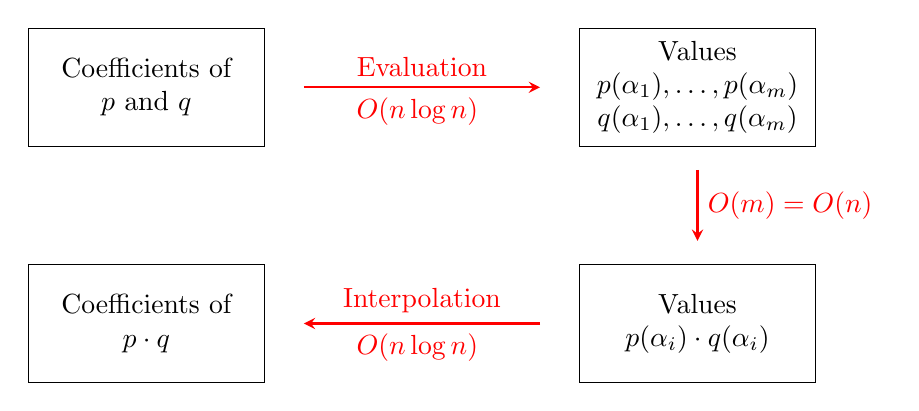
\begin{tikzpicture}[every text node part/.style={align=center}]
				\foreach \x in {0, 7}
				\foreach \y in {0, 3}
				{
					\draw (\x, \y) -- (\x+3, \y) -- (\x+3, \y+1.5) -- (\x, \y+1.5) -- cycle;
				}
				\draw node at (1.5, 0.75) {Coefficients of \\ \( p \cdot q \)};
				\draw node at (1.5, 3.75) {Coefficients of \\ \( p \) and \( q \) };
				\draw node at (8.5, 0.75) {Values \\ \( p(\alpha_i) \cdot q(\alpha_i) \) };
				\draw node at (8.5, 3.75) {Values \\ \( p(\alpha_1), \dots, p(\alpha_m) \) \\ \( q(\alpha_1), \dots, q(\alpha_m) \) };
				\draw[-stealth, red, thick] (3.5, 3.75) --node[midway, above] {Evaluation} node[midway, below] 
					{\( O(n \log n) \) } (6.5, 3.75); 
				\draw[-stealth, red, thick] (8.5, 2.7) -- node[midway, right] {\( O(m) = O(n) \) } (8.5, 1.8);
				\draw[-stealth, red, thick] (6.5, 0.75) -- node[midway, above] {Interpolation} node[midway, below] 
					{\( O(n \log n) \) } (3.5, 0.75);
			\end{tikzpicture}
		\end{center}
		If we can do this whole sequence, then that gives us an efficient multiplication algorithm. However, the evaluation step 
		still takes \( O(m \cdot n) = O(n^2) \) time, so how can we possibly get this down to \( O(n \log n) \)? The secret 
		lies in how we pick \( \alpha_1, \dots, \alpha_m \) -- it is possible to pick them in such a way that the evaluation 
		step takes \( O(n \log n) \) time. Same goes for interpolation. 

		How do we pick \( \alpha_1, \dots, \alpha_m \)? We use complex numbers!
\end{itemize}

\subsection{Complex Numbers}
\begin{itemize}
	\item A complex number is any number of the form \( a + bi \), where \( i = \sqrt{-1}  \). \( a \) represents the real part, and 
		\( b \) represents the imaginary part of the number. We can add complex numbers:
		\[
			(1 + 2i) + (3 + 4i) = (1 + 3) + (2 + 4)i = 4 + 6i
		\] 
		so the real parts add and the imaginary part also adds. To multiply:
		\[
			(1 + 2i) \cdot (3 + 4i) = 1 \cdot 3 + 1 \cdot 4i + 2i \cdot 3 + 2i \cdot 4i = 3 + 10i - 8 = -5 + 10i
		\] 
		Recall that since \( i = \sqrt{-1}  \), then  \( i^2 = -1 \). 
	\item We can also represent complex numbers on the complex plane. A number \( a + bi \) corresponds to  \( (a, b) \) on the 
		complex plane. We can also represent it using polar coordinates, using a radius \( r \) and an angle \( \theta \)
		\begin{center}
			\begin{tikzpicture}
				\draw (-3, 0) -- (3, 0) node[above] {real};
				\draw (0, -3) -- (0, 3) node[above right] {imaginary};
				\draw[red] (0, 0) -- node[midway, above] {\( r \) } (1.8, 1.4) node[above right, black] {\( (a, b) \) }; 
				\filldraw[red] (1.8, 1.4) circle (2pt); 
				\draw[red] (1, 0) arc (0:37.87:1) node[midway, right]{\( \theta \) };
			\end{tikzpicture}
		\end{center}
		With this construction, we can relate polar to cartesian with the relations
		\begin{align*}
			a &= r\cos\theta \\
			b&= r \sin \theta 
		\end{align*}
		For today, we'll only consider points with \( r = 1 \). This means that we basically forget about \( r \), and only 
		worry about \( \theta \). So with \( r = 1 \), then we have:
		\begin{align*}
			a &=  \cos \theta \\
			b &=  \sin \theta 
		\end{align*}
		And since \( r = 1 \), we'll be dealing with points on the \textbf{unit circle}.
	\item Consider two complex numbers, the first specified by \( \theta_1 \), and the other specified by \( \theta_2 \) (both 
		having \( r = 1 \) ). Then, we define the product of the two to be specified by \( \theta_1 + \theta_2 \). To multiply, 
		we just add the angles.
\end{itemize}
\subsubsection{Roots of Unity}
\begin{itemize}
	\item The \( n \)-th root of unity is a solution to the equation \( x^{n} = 1 \). So the second roots of uhnity are solutions 
		to the equation \( x^2 = 1 \), which are \( \pm 1 \). The 4-th roots of unity are solutions to \( x^{4} = 1 \), 
		which are \( \{1, -1, i, -i\}  \). 
	\item In general, the \( n \)-th roots of unity will have \( n \) distinct solutions. 
	\item Graphically, the \( n \)-th roots of unity correspond to \( n \) equally spaced points placed on the unit circle.   
	\item When we talk about the roots of unity, we will use \( \omega_0 \) through \( \omega_{n-1} \) to label them. In particular, 
		we'll focus on \( \omega_1 \).
		\begin{itemize}
			\item Note that \( \omega_1 \) always sits at an angle of \( \frac{2\pi}{n} \) for the \( n \)-th roots of unity, due 
				to the even spacing.
			\item Note that \( \omega_2 = \omega_1 \cdot \omega_1 \), since multiplying is equivalent to adding the angles together.
				Therefore, we have the relation that \( \omega_i = \omega_1^{i} \), which we will call the \textbf{Generator Fact}. 
		\end{itemize}
	\item So this gives us a nice formula for the \( n \)-th roots of unity: they will always sit at angles \( k\theta \), where 
		\( \theta = 2\pi / n \). As angles, this is represented as the set: \( \{\cos(k\ell) + i\sin(k\ell) | \ell= 0, 1, \dots, 
		n - 1\}  \).  
\end{itemize}
\subsubsection{Square Roots}
\begin{itemize}
	\item When we take a square root, remember that they always come in pairs of \( \pm \sqrt{a}  \). So to get the second 
		roots of unity, we find the square roots of 1, which are \(  \pm 1 \). To get the 4-th roots of unity, then we just need 
		to take the square roots of the previous roots of unity. 

		In general, if we take the square roots of the \( n \)-th root of unity, then we generate the \( 2n \)-th root of unity. 
		Conversely, if we square the roots of unity then we get the \( n / 2 \)-th roots of unity. 

		This is the magical fact that we will leverage for the following lecture: squaring the \( n \)-th roots gives us 
		the \( n / 2 \)-th roots of unity. This is not true for most numbers! For instance, squaring the set \( \{1, 3, 5, 7\}  \)
		gives \( \{1, 8, 25, 49\}  \), which still contains the same number of elements as the original set!
\end{itemize}
\subsection{Fast Polynomial Multiplication Algorithm (Preview)}
\begin{itemize}
	\item Recall the evaluation step in our polynomial multiplication: \( p \cdot q \) is degree \( 2n - 2 \), so we need 
		\( m \ge 2n - 1 \). Let \( m \) be the first power of 2 such that \( m \ge  2n - 1 \). Then, we will evaluate \( p \) 
		and \( q \) on the \( m \)-th roots of unity in time \( O(m \log m) = O(n \log n)\), 
		using the \textbf{Fast Fourier Transform}.  
\end{itemize}
